\documentclass[aspectratio=169,11pt]{beamer}

\usepackage[utf8]{inputenc}
\usepackage[T1]{fontenc}
\usepackage{lmodern}
\usepackage{booktabs}
\usepackage{tabularx}
\usepackage{array}
\usepackage{tikz}
\usetikzlibrary{shapes.geometric,shapes.multipart,arrows.meta,positioning,fit,calc,backgrounds}

% =====================================================================
%  EDIT THESE LINES ONLY - used by both the report and the slides.
%  After editing, recompile (see docs/README.md).
% =====================================================================
\newcommand{\ProjectTitle}{SmartDock: A Multi-Tenant Dock Appointment Scheduling and Yard Management System for Warehouses and Distribution Centres}
\newcommand{\ProjectShortTitle}{SmartDock}
\newcommand{\StudentName}{[Student Name]}
\newcommand{\RegisterNumber}{[Register Number]}
\newcommand{\GuideName}{[Guide Name, Designation]}
\newcommand{\Programme}{[Programme, e.g. MBA / B.Tech]}
\newcommand{\Department}{[Department Name]}
\newcommand{\Institution}{[College / University Name]}
\newcommand{\InstitutionPlace}{[City]}
\newcommand{\AcademicYear}{2026--2027}
\newcommand{\SubmissionMonth}{November 2026}
\newcommand{\Course}{Supply Chain Management -- Final Project}
% Links (already filled in)
\newcommand{\GitHubURL}{https://github.com/RamaguruS/Dock}
\newcommand{\LiveURL}{https://smartdock.onrender.com}

% Shared colours and TikZ styles for the report and the slides
\definecolor{brand}{HTML}{6D28D9}
\definecolor{ink}{HTML}{1F2937}
\definecolor{muted}{HTML}{6B7280}
\definecolor{boxbg}{HTML}{F5F3FF}
\tikzset{
  blk/.style={draw=ink!70, rounded corners=3pt, fill=white, align=center, font=\small, minimum height=0.9cm, inner sep=4pt},
  layer/.style={draw=brand!60, fill=boxbg, rounded corners=5pt, inner sep=7pt},
  lbl/.style={font=\scriptsize\bfseries\color{brand}, anchor=north west},
  arr/.style={-{Stealth[length=2.2mm]}, draw=ink!70, thick},
  darr/.style={{Stealth[length=2.2mm]}-{Stealth[length=2.2mm]}, draw=ink!70, thick},
  ent/.style={draw=ink!80, fill=white, minimum width=2.6cm, minimum height=1cm, align=center, font=\small\bfseries},
  proc/.style={circle, draw=brand, fill=boxbg, align=center, font=\scriptsize\bfseries, minimum size=2.2cm, inner sep=1pt},
  store/.style={draw=ink!70, fill=gray!8, minimum width=3.0cm, minimum height=0.7cm, font=\scriptsize\bfseries, path picture={\draw[ink!70] (path picture bounding box.north west) -- (path picture bounding box.south west);}},
  flow/.style={-{Stealth[length=2mm]}, draw=ink!60, font=\scriptsize, align=center},
}

\graphicspath{{../figures/}}

% ---------------------------------------------------------------- theme
\usetheme{default}
\setbeamertemplate{navigation symbols}{}
\setbeamercolor{structure}{fg=brand}
\setbeamercolor{frametitle}{fg=white,bg=brand}
\setbeamercolor{title}{fg=ink}
\setbeamercolor{normal text}{fg=ink}
\setbeamercolor{alerted text}{fg=brand}
\setbeamerfont{frametitle}{size=\large,series=\bfseries}
\setbeamertemplate{frametitle}{%
  \nointerlineskip
  \begin{beamercolorbox}[wd=\paperwidth,ht=2.4ex,dp=1.2ex,leftskip=0.6cm]{frametitle}
    \insertframetitle
  \end{beamercolorbox}}
\setbeamertemplate{itemize item}{\color{brand}$\blacktriangleright$}
\setbeamertemplate{itemize subitem}{\color{brand}--}
\setbeamertemplate{footline}{%
  \hbox{\begin{beamercolorbox}[wd=\paperwidth,ht=2.4ex,dp=1ex,leftskip=0.6cm,rightskip=0.6cm]{normal text}%
    \tiny\color{muted}\ProjectShortTitle{} --- \StudentName\hfill\insertframenumber/\inserttotalframenumber
  \end{beamercolorbox}}}

\newcommand{\diagram}[2][0.78]{\begin{center}\resizebox{!}{#1\textheight}{\input{../diagrams/#2}}\end{center}}
\newcommand{\shot}[2][0.72]{\begin{center}\fbox{\includegraphics[height=#1\textheight]{#2}}\end{center}}

\begin{document}

% ================================================================ 1 title
\begin{frame}[plain]
\begin{tikzpicture}[remember picture,overlay]
  \fill[brand] (current page.north west) rectangle ([yshift=-0.35cm]current page.north east);
  \fill[boxbg] (current page.south west) rectangle ([yshift=1.2cm]current page.south east);
\end{tikzpicture}
\vspace{0.2cm}
\begin{center}
{\small\color{muted}\Institution\ $\cdot$ \Department}\\[0.5cm]
{\Huge\bfseries\color{brand}\ProjectShortTitle}\\[0.25cm]
{\large\color{ink}Dock Appointment Scheduling \& Yard Management\\for Warehouses and Distribution Centres}\\[0.7cm]
\begin{tabular}{rl}
\textbf{Student} & \StudentName\ (\RegisterNumber)\\
\textbf{Guide} & \GuideName\\
\textbf{Programme} & \Programme, \Department\\
\textbf{Academic year} & \AcademicYear\\
\end{tabular}\\[0.4cm]
{\small\color{muted}\Course}
\end{center}
\end{frame}

% ================================================================ 2 outline
\begin{frame}{Outline}
\begin{columns}[T]
\column{0.48\textwidth}
\begin{enumerate}\small
  \item Introduction: IT in supply chains
  \item Problem statement
  \item Objectives
  \item Scope and limitations
  \item Background and literature survey
  \item Gap and proposed solution
  \item System architecture
  \item DFD, use case and ER diagrams
  \item Technology stack
  \item Modules
\end{enumerate}
\column{0.48\textwidth}
\begin{enumerate}\small\setcounter{enumi}{10}
  \item Implementation details
  \item Screenshots and live demo
  \item Testing and validation
  \item Results and discussion
  \item Benefits and applications
  \item Conclusion
  \item Future enhancements
  \item References
\end{enumerate}
\end{columns}
\end{frame}

% ================================================================ 3 intro
\begin{frame}{Introduction: Role of IT in Modern Supply Chains}
\begin{columns}[T]
\column{0.55\textwidth}
\begin{itemize}
  \item Supply chains compete on \alert{coordination} between independent partners --- suppliers, carriers, warehouses.
  \item IT provides:
  \begin{itemize}
    \item \textbf{Visibility} --- one shared, real-time picture
    \item \textbf{Synchronisation} --- partners work to one plan
    \item \textbf{Automation} --- rules replace phone calls
    \item \textbf{Measurement} --- KPIs for continuous improvement
  \end{itemize}
  \item ERP, WMS, TMS, YMS \ldots\ but the \alert{loading dock} --- the hand-over between transport and warehouse --- is often still managed by phone and whiteboard.
\end{itemize}
\column{0.42\textwidth}
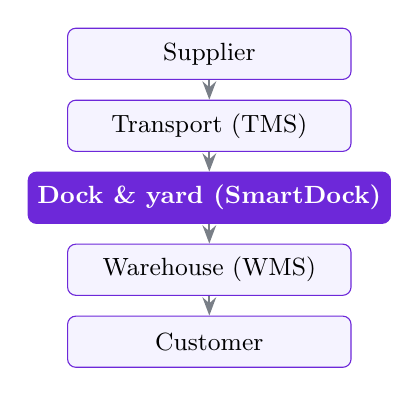
\begin{tikzpicture}[node distance=0.25cm, b/.style={draw=brand, fill=boxbg, rounded corners=3pt, minimum width=3.6cm, minimum height=0.65cm, font=\small}]
  \node[b] (s) {Supplier};
  \node[b, below=of s] (t) {Transport (TMS)};
  \node[b, below=of t, fill=brand, text=white, font=\small\bfseries] (d) {Dock \& yard (SmartDock)};
  \node[b, below=of d] (w) {Warehouse (WMS)};
  \node[b, below=of w] (c) {Customer};
  \foreach \a/\b in {s/t,t/d,d/w,w/c} \draw[-{Stealth}, thick, ink!60] (\a) -- (\b);
\end{tikzpicture}
\end{columns}
\end{frame}

% ================================================================ 4 problem
\begin{frame}{Problem Statement}
\begin{columns}[T]
\column{0.55\textwidth}
Without dock appointments:
\begin{itemize}
  \item Trucks arrive at the same \alert{peak hours} $\rightarrow$ yard queues, idle docks at other times
  \item Driver \alert{detention} and unplanned dock labour
  \item \alert{Double-booking} and wrong doors (reefer, hazmat)
  \item No record of who is late or never arrives
  \item No data: utilisation? busiest hours? turnaround?
\end{itemize}
\column{0.42\textwidth}
\begin{block}{Problem}
\small Build a web platform where warehouses publish dock capacity and carriers self-book \textbf{compatible, conflict-free} appointments, while yard events are captured to measure and improve \textbf{utilisation, punctuality and turnaround} --- securely, for many warehouses and carriers.
\end{block}
\end{columns}
\end{frame}

% ================================================================ 5 objectives
\begin{frame}{Objectives}
\begin{columns}[T]
\column{0.5\textwidth}
\begin{enumerate}\small
  \item Multi-tenant platform with per-warehouse carrier approval
  \item Configurable scheduling: hours, 15--90 min slots, buffers, holidays, maintenance
  \item Match loads to docks: inbound/outbound, trailer type, hazmat
  \item \alert{Guarantee} slot capacity under concurrent requests
  \item Recurring bookings, rescheduling, automatic waitlist
\end{enumerate}
\column{0.5\textwidth}
\begin{enumerate}\small\setcounter{enumi}{5}
  \item Digitise yard execution; detect late arrivals and no-shows
  \item Carrier reliability score and operational KPIs
  \item Audit trail and notifications (in-app, e-mail, SMS)
  \item Cloud deployment, automated tests, simulation study
\end{enumerate}
\end{columns}
\end{frame}

% ================================================================ 6 scope
\begin{frame}{Scope and Limitations}
\begin{columns}[T]
\column{0.48\textwidth}
\textbf{Scope}
\begin{itemize}\small
  \item Users: warehouse managers, carriers, super admin
  \item Full appointment lifecycle, waitlist, yard events, KPIs, audit, notifications, exports
  \item One cloud service + managed database, any browser
  \item Demo data: 2 DCs, 5 typed docks, 6 carriers, 5 weeks
\end{itemize}
\column{0.48\textwidth}
\textbf{Limitations}
\begin{itemize}\small
  \item No ERP/WMS/TMS integration (PO/ASN entered manually)
  \item Gate events recorded manually (no ANPR / IoT)
  \item Fixed slot length per site
  \item Super-admin role has no UI yet
  \item Evaluation on generated / simulated data
  \item Free hosting: cold start, small CPU
\end{itemize}
\end{columns}
\end{frame}

% ================================================================ 7 background
\begin{frame}{Background: Docks, Yards and Dock KPIs}
\begin{columns}[T]
\column{0.5\textwidth}
\begin{itemize}\small
  \item \textbf{Dock door}: inbound (receiving) or outbound (shipping); capacity per period
  \item \textbf{Equipment}: dry van, \alert{reefer} (cold chain), flatbed, container; \alert{hazmat} needs certified bays
  \item \textbf{Yard}: where trucks wait before / after docking
  \item \textbf{Appointment}: a reserved door for a time window
\end{itemize}
\column{0.47\textwidth}
\begin{block}{Key performance indicators}
\small
\begin{itemize}
  \item Dock utilisation = booked $\div$ offered truck-slots
  \item On-time arrival rate
  \item No-show rate
  \item Turnaround = yard wait + dock time
\end{itemize}
\end{block}
\end{columns}
\end{frame}

% ================================================================ 8 literature
\begin{frame}{Literature Survey and Existing Systems}
\footnotesize
\begin{itemize}
  \item Port \textbf{truck appointment systems} reduce congestion when enforced (Giuliano \& O'Brien 2007; Huynh \& Walton 2008; Zehendner \& Feillet 2014; Phan \& Kim 2015)
  \item Receiving/shipping and \textbf{cross-dock scheduling} drive warehouse throughput (Gu et al.\ 2007; Boysen \& Fliedner 2010)
  \item \textbf{Write skew} can double-book under concurrency (Kleppmann 2017)
\end{itemize}
\vspace{2pt}
\scriptsize
\begin{tabularx}{\textwidth}{>{\raggedright\arraybackslash}p{2.6cm}*{5}{>{\centering\arraybackslash}X}}
\toprule
& Phone / spreadsheet & Port TAS & Dock-scheduling SaaS & WMS/YMS suite & \textbf{SmartDock}\\
\midrule
Carrier self-service & No & Yes & Yes & Partial & \textbf{Yes}\\
Capacity enforced & Manual & Yes & Yes & Yes & \textbf{Atomic, multi-server}\\
Dock-type / hazmat & Manual & Limited & Varies & Yes & \textbf{Yes}\\
Waitlist / recurring & No & Varies & Varies & Varies & \textbf{Yes}\\
Scorecard \& KPIs & No & Terminal KPIs & Yes & Yes & \textbf{Yes}\\
Cost & Effort & Port-run & Subscription & High & \textbf{Free, open source}\\
\bottomrule
\end{tabularx}
\end{frame}

% ================================================================ 9 gap
\begin{frame}{Gap in Existing Systems and Proposed Solution}
\begin{columns}[T]
\column{0.47\textwidth}
\textbf{Gap}
\begin{itemize}\small
  \item SMEs stuck between manual methods and expensive enterprise suites
  \item Port systems are not built for multi-tenant warehouses with mixed docks
  \item Simple calendars ignore compatibility, capacity and concurrency
  \item Booking separated from execution $\rightarrow$ no KPIs, no accountability
\end{itemize}
\column{0.5\textwidth}
\textbf{SmartDock}
\begin{itemize}\small
  \item Per-warehouse rules and carrier access
  \item Only compatible docks and valid slots; \alert{concurrency-safe} capacity
  \item Full lifecycle: request $\rightarrow$ approve $\rightarrow$ gate $\rightarrow$ dock $\rightarrow$ depart; reschedule, series, waitlist
  \item KPIs, reliability score, reports, audit, notifications
  \item Free, open source, one-file cloud deployment
\end{itemize}
\end{columns}
\end{frame}

% ================================================================ 10 architecture
\begin{frame}{System Architecture}
\diagram[0.86]{arch}
\end{frame}

% ================================================================ 11-13 diagrams
\begin{frame}{Context Diagram (DFD Level 0)}
\diagram[0.8]{dfd0}
\end{frame}

\begin{frame}{Appointment Lifecycle (State Machine)}
\begin{center}\resizebox{\textwidth}{!}{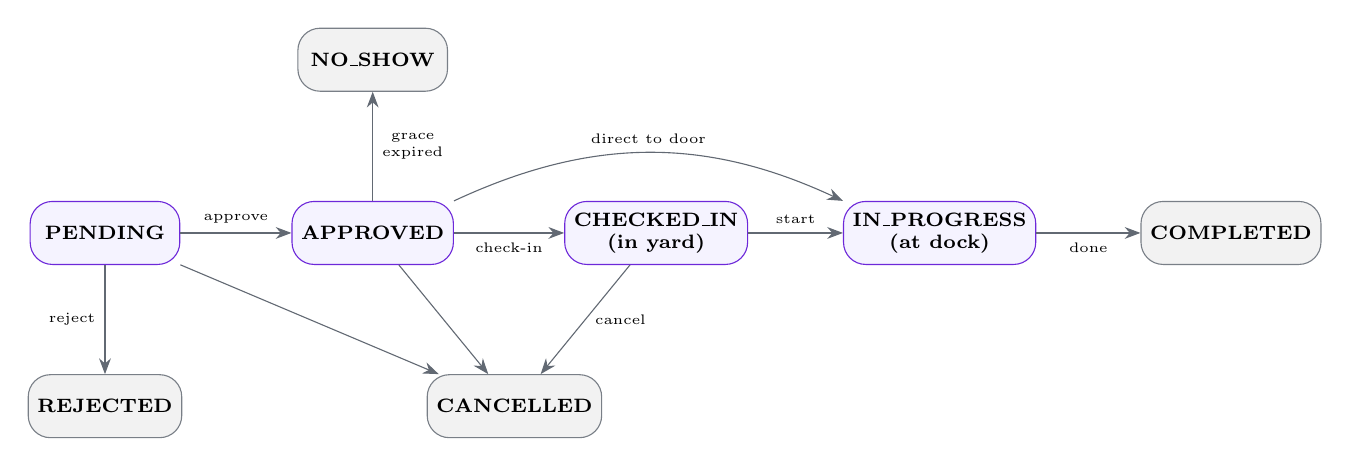
\begin{tikzpicture}[st/.style={rounded corners=8pt, draw=brand, fill=boxbg, font=\scriptsize\bfseries, minimum width=1.9cm, minimum height=0.8cm, align=center},
  term/.style={st, draw=ink!60, fill=gray!10}, t/.style={-{Stealth[length=2mm]}, draw=ink!70, font=\tiny, align=center}]
  \node[st] (p) at (0,0) {PENDING};
  \node[st] (a) at (3.4,0) {APPROVED};
  \node[st] (c) at (7.0,0) {CHECKED\_IN\\(in yard)};
  \node[st] (i) at (10.6,0) {IN\_PROGRESS\\(at dock)};
  \node[term] (d) at (14.3,0) {COMPLETED};
  \node[term] (r) at (0,-2.2) {REJECTED};
  \node[term] (x) at (5.2,-2.2) {CANCELLED};
  \node[term] (n) at (3.4,2.2) {NO\_SHOW};
  \draw[t] (p) -- node[above]{approve} (a);
  \draw[t] (a) -- node[below]{check-in} (c);
  \draw[t] (c) -- node[above]{start} (i);
  \draw[t] (i) -- node[below]{done} (d);
  \draw[t] (a.north east) to[bend left=25] node[above]{direct to door} (i.north west);
  \draw[t] (p) -- node[left]{reject} (r);
  \draw[t] (p) -- (x);
  \draw[t] (a) -- (x);
  \draw[t] (c) -- node[right]{cancel} (x);
  \draw[t] (a) -- node[right]{grace\\expired} (n);
\end{tikzpicture}
}\end{center}
\small COMPLETED, CANCELLED, REJECTED and NO\_SHOW are terminal: released capacity can never be silently re-occupied. Late / on-time is recorded at gate check-in; NO\_SHOW is set automatically after the grace period.
\end{frame}

\begin{frame}{Data Flow Diagram (Level 1)}
\diagram[0.8]{dfd1}
\end{frame}

\begin{frame}{Use Case Diagram}
\diagram[0.84]{usecase}
\end{frame}

\begin{frame}{Entity--Relationship Diagram}
\diagram[0.84]{er}
\end{frame}

% ================================================================ 14 stack
\begin{frame}{Technology Stack}
\small
\begin{tabularx}{\textwidth}{>{\bfseries\raggedright\arraybackslash}p{3.1cm}X}
\toprule
Language & TypeScript (client and server)\\
Frontend & React 19, Vite, Tailwind CSS, React Query, React Hook Form + Zod, jsPDF\\
Backend & Node.js 22, Express, Zod validation, JWT, bcrypt, rate limiting, Winston\\
Database & MongoDB Atlas (replica set), Mongoose --- transactions, indexes, aggregations\\
APIs & REST/JSON ($\approx$40 endpoints); Resend (e-mail), Twilio (SMS)\\
Cloud \& DevOps & Render (Blueprint \texttt{render.yaml}, auto-deploy from GitHub), Atlas M0\\
Testing \& tools & In-memory replica set + 2 API instances (58 checks); Git, VS Code, Python, \LaTeX\\
\bottomrule
\end{tabularx}
\end{frame}

% ================================================================ 15 modules
\begin{frame}{Modules}
\small
\begin{columns}[T]
\column{0.5\textwidth}
\begin{enumerate}
  \item \textbf{Identity \& access} --- roles, per-warehouse approval
  \item \textbf{Site \& docks} --- doors, equipment, hours, rules, holidays, maintenance
  \item \textbf{Scheduling engine} --- slot grid, availability, atomic reservation
  \item \textbf{Booking} --- wizard, weekly series, reschedule
  \item \textbf{Waitlist} --- FIFO auto-assignment
\end{enumerate}
\column{0.5\textwidth}
\begin{enumerate}\setcounter{enumi}{5}
  \item \textbf{Yard execution} --- gate check-in, dock start, complete, no-show
  \item \textbf{Carrier performance} --- reliability score, tiers A--D
  \item \textbf{Analytics} --- KPIs, heatmap, CSV/PDF, gate sheet
  \item \textbf{Notifications} --- in-app, e-mail, SMS, reminders
  \item \textbf{Audit trail} --- who did what, when
\end{enumerate}
\end{columns}
\end{frame}

% ================================================================ 16-17 implementation
\begin{frame}{Implementation: Key Logic}
\begin{columns}[T]
\column{0.52\textwidth}
\small
\textbf{Slot grid} (site time zone, DST-safe)
\[ s_k = o + k(L+B),\quad e_k = s_k + L \le c \]
$L$ = slot length, $B$ = buffer (30 + 15 $\Rightarrow$ 08:00, 08:45, \ldots)

\textbf{Compatibility}: direction matches (or both) $\wedge$ trailer type supported $\wedge$ (not hazmat $\vee$ certified)

\textbf{Arrival}: late if check-in $-$ slot start $>$ threshold (15 min)

\textbf{Background jobs} (every minute): no-shows, expiry, 24 h reminders, waitlist expiry
\column{0.45\textwidth}
\begin{block}{Carrier reliability score}
\[ R = \frac{\text{on-time} + 0.5\times\text{late}}{\text{arrivals} + \text{no-shows}} \times 100 \]
\small A $\ge$ 90 $\cdot$ B $\ge$ 75 $\cdot$ C $\ge$ 50 $\cdot$ D $<$ 50
\end{block}
\begin{block}{Waitlist}
\small Capacity released (cancel / reject / reschedule) $\Rightarrow$ oldest compatible waiting carrier booked automatically, inside the same transaction.
\end{block}
\end{columns}
\end{frame}

\begin{frame}{Implementation: Concurrency-Safe Capacity Reservation}
\begin{columns}[c]
\column{0.5\textwidth}
\resizebox{\textwidth}{!}{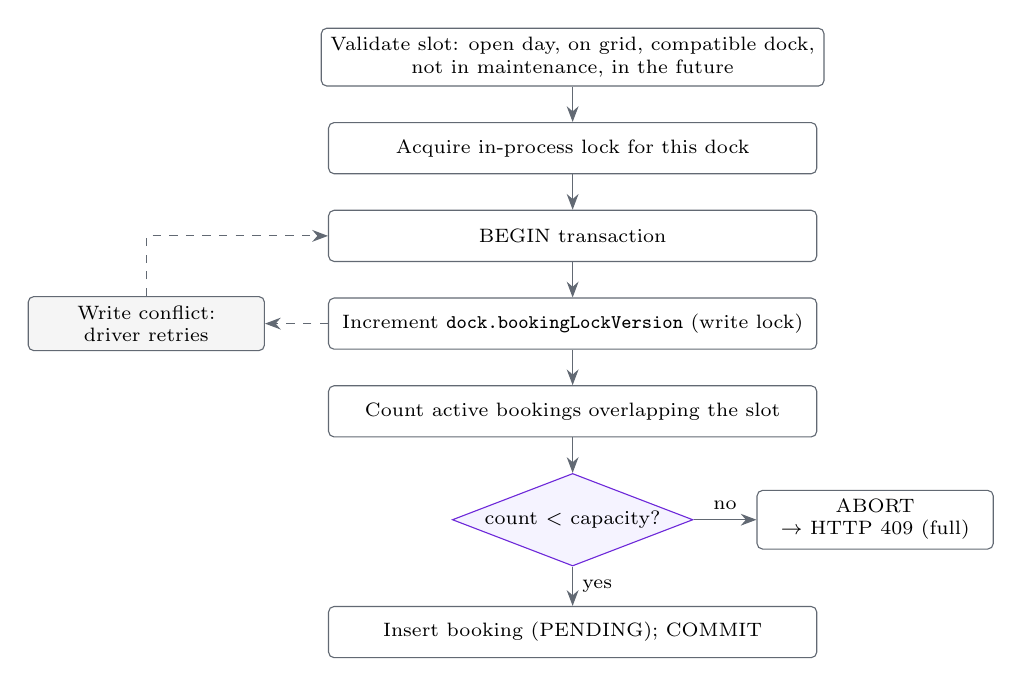
\begin{tikzpicture}[node distance=0.45cm, every node/.style={font=\scriptsize}]
  \tikzset{fb/.style={draw=ink!70, rounded corners=2pt, fill=white, align=center, minimum width=6.2cm, minimum height=0.65cm},
           fd/.style={diamond, aspect=2.6, draw=brand, fill=boxbg, align=center, inner sep=1pt},
           fa/.style={-{Stealth[length=2mm]}, draw=ink!70}}
  \node[fb] (a) {Validate slot: open day, on grid, compatible dock,\\not in maintenance, in the future};
  \node[fb, below=of a] (b) {Acquire in-process lock for this dock};
  \node[fb, below=of b] (c) {BEGIN transaction};
  \node[fb, below=of c] (d) {Increment \texttt{dock.bookingLockVersion} (write lock)};
  \node[fb, below=of d] (e) {Count active bookings overlapping the slot};
  \node[fd, below=of e] (f) {count $<$ capacity?};
  \node[fb, below=0.5cm of f] (g) {Insert booking (PENDING); COMMIT};
  \node[fb, right=0.8cm of f, minimum width=3.0cm] (h) {ABORT\\$\rightarrow$ HTTP 409 (full)};
  \node[fb, left=0.8cm of d, minimum width=3.0cm, fill=gray!8] (r) {Write conflict:\\driver retries};
  \draw[fa] (a) -- (b); \draw[fa] (b) -- (c); \draw[fa] (c) -- (d); \draw[fa] (d) -- (e); \draw[fa] (e) -- (f);
  \draw[fa] (f) -- node[right]{yes} (g); \draw[fa] (f) -- node[above]{no} (h);
  \draw[fa, dashed] (d.west) -- (r.east); \draw[fa, dashed] (r.north) |- (c.west);
\end{tikzpicture}
}
\column{0.48\textwidth}
\small
\begin{itemize}
  \item Naive ``count, then insert'' lets two requests both see a free place (\alert{write skew})
  \item Even a transaction alone does not help: each reads its own snapshot
  \item SmartDock: every reservation \alert{writes the dock document} first $\Rightarrow$ concurrent transactions conflict, the database retries them, the retry sees the booking
  \item Plus an in-process lock per dock
  \item Same routine for bookings, series, reschedules, waitlist
\end{itemize}
\end{columns}
\end{frame}

% ================================================================ 18-21 screenshots
\begin{frame}{Screens: Yard Schedule (Warehouse Manager)}
\shot[0.8]{yard_schedule.jpg}
\end{frame}

\begin{frame}{Screens: Docks and Carrier Scorecard}
\begin{columns}[c]
\column{0.5\textwidth}\centering\fbox{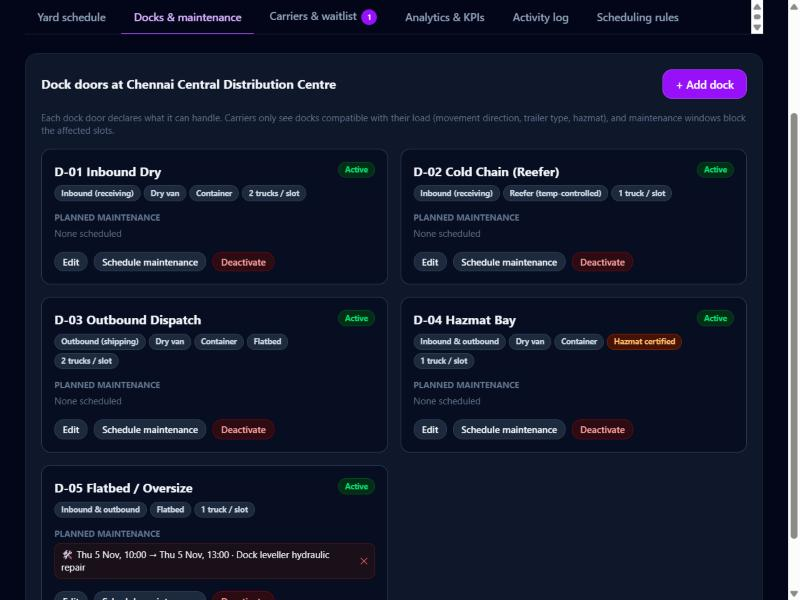
\includegraphics[width=0.95\textwidth]{docks.jpg}}
\column{0.5\textwidth}\centering\fbox{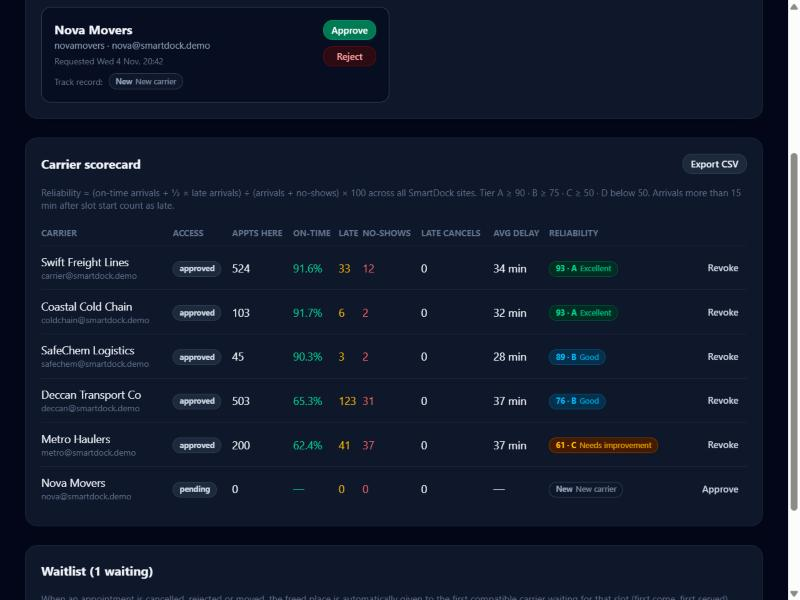
\includegraphics[width=0.95\textwidth]{carriers.jpg}}
\end{columns}
\end{frame}

\begin{frame}{Screens: Analytics, Rules and Audit}
\begin{columns}[c]
\column{0.33\textwidth}\centering\fbox{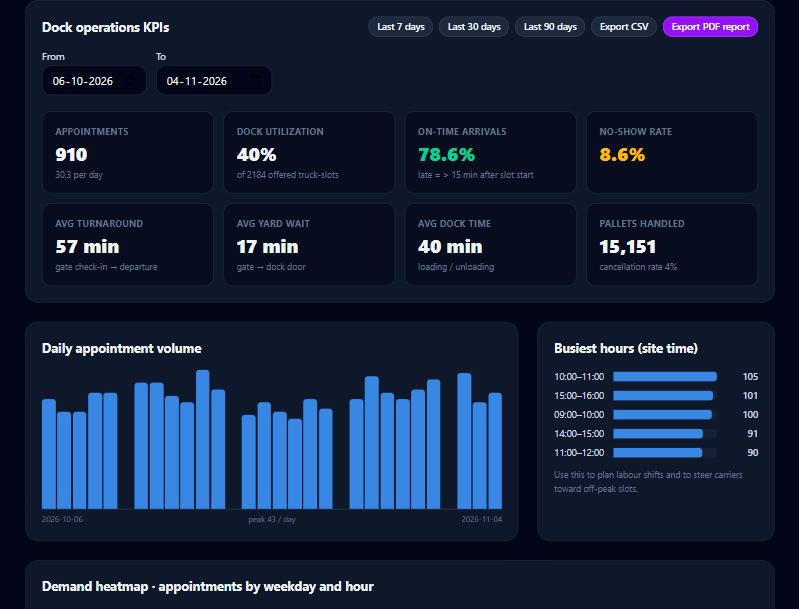
\includegraphics[width=0.95\textwidth]{analytics_kpis.jpg}}\\{\scriptsize KPIs}
\column{0.33\textwidth}\centering\fbox{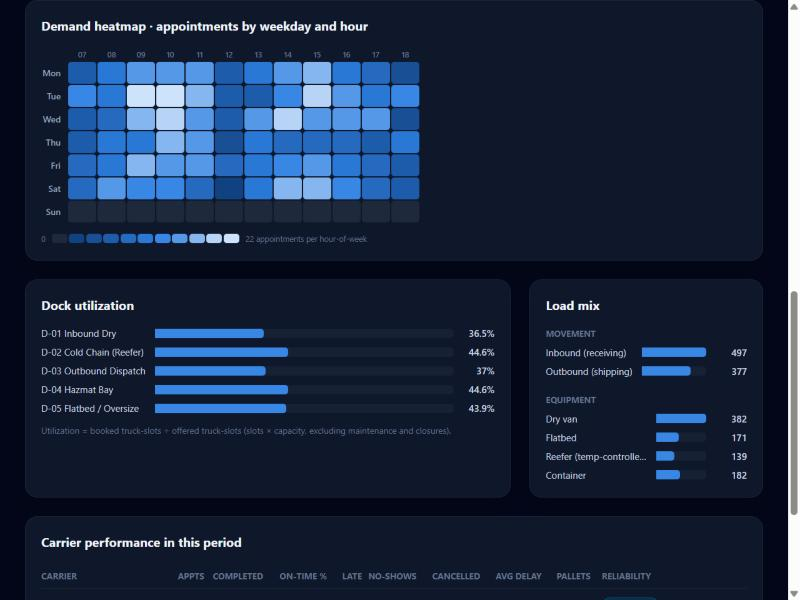
\includegraphics[width=0.95\textwidth]{analytics_heatmap.jpg}}\\{\scriptsize Heatmap \& utilisation}
\column{0.33\textwidth}\centering\fbox{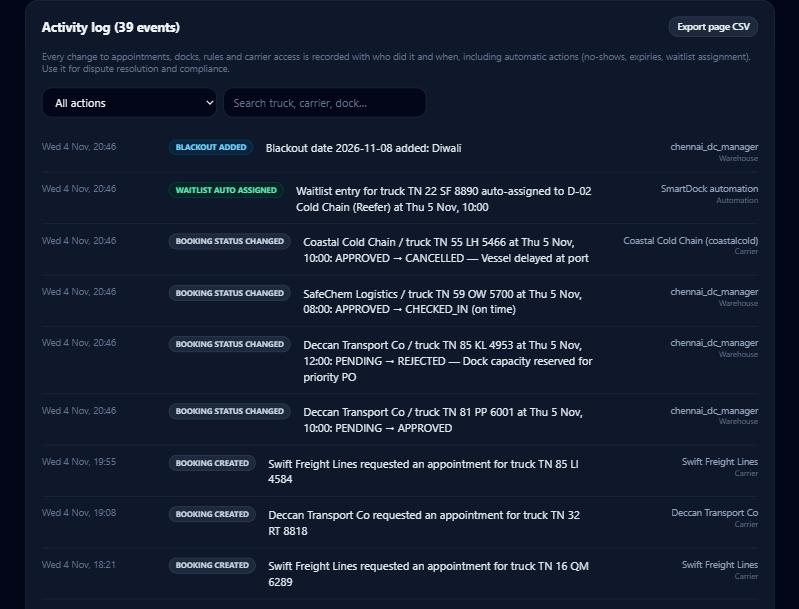
\includegraphics[width=0.95\textwidth]{activity_log.jpg}}\\{\scriptsize Activity log}
\end{columns}
\end{frame}

\begin{frame}{Screens: Carrier Booking Wizard}
\begin{columns}[c]
\column{0.33\textwidth}\centering\fbox{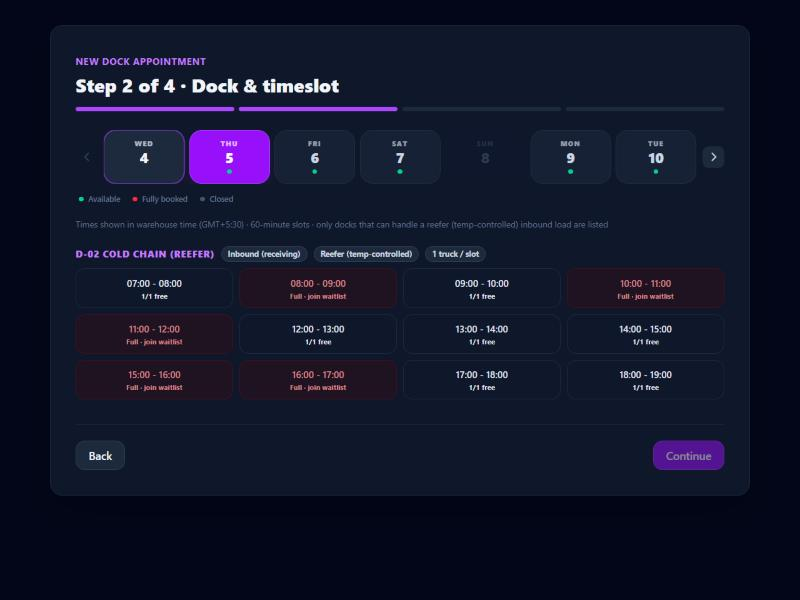
\includegraphics[width=0.95\textwidth]{booking_slots.jpg}}\\{\scriptsize Compatible docks only; waitlist on full slots}
\column{0.33\textwidth}\centering\fbox{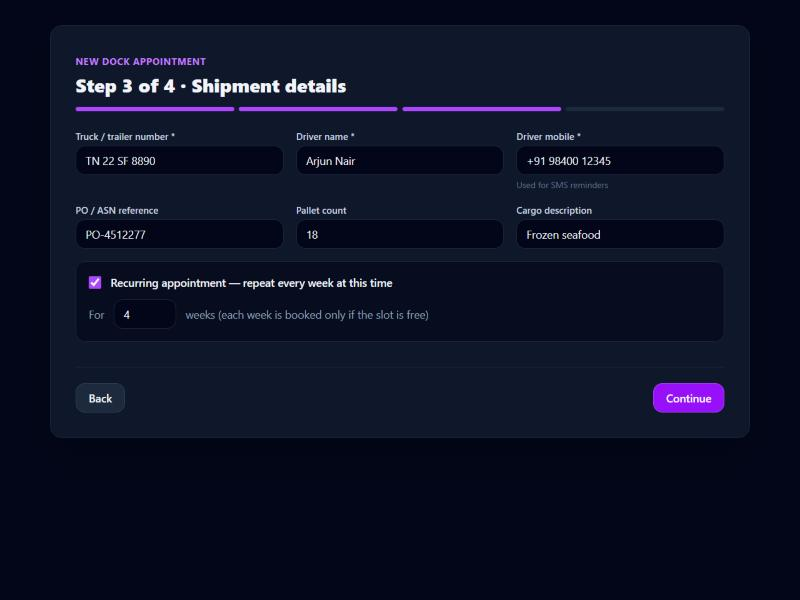
\includegraphics[width=0.95\textwidth]{booking_details.jpg}}\\{\scriptsize Truck, driver, PO/ASN, weekly series}
\column{0.33\textwidth}\centering\fbox{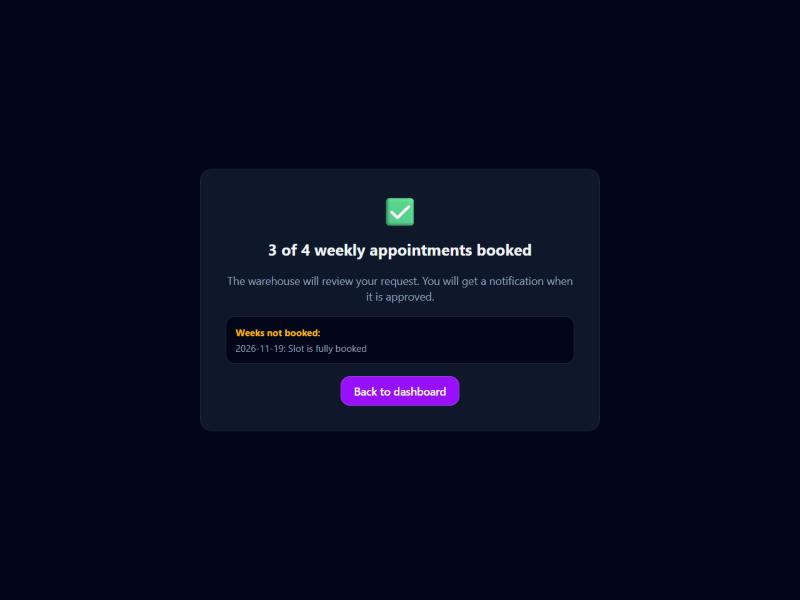
\includegraphics[width=0.95\textwidth]{booking_result.jpg}}\\{\scriptsize 3 of 4 weeks booked}
\end{columns}
\end{frame}

\begin{frame}{Live Demo}
\begin{columns}[T]
\column{0.5\textwidth}
\begin{block}{Links}
\small
\textbf{Live:} \url{\LiveURL}\\
\textbf{Code:} \url{\GitHubURL}\\[3pt]
Manager: \texttt{admin@smartdock.demo}\\
Carrier: \texttt{carrier@smartdock.demo}\\
Password: \texttt{Demo@123}
\end{block}
\column{0.47\textwidth}
\textbf{Demo flow}
\begin{enumerate}\small
  \item Carrier books a reefer slot, weekly series; joins a waitlist
  \item Manager approves $\rightarrow$ gate check-in $\rightarrow$ dock $\rightarrow$ complete
  \item Docks, maintenance, rules, holidays
  \item Analytics, PDF report, gate sheet, audit log
  \item New carrier (Nova Movers) approval
\end{enumerate}
\end{columns}
\end{frame}

% ================================================================ 22 testing
\begin{frame}{Testing and Validation}
\begin{columns}[T]
\column{0.5\textwidth}
\small
\begin{itemize}
  \item 58 automated end-to-end checks on an in-memory \textbf{replica set} with \textbf{two} API servers --- all pass
  \item Security \& tenancy, capacity \& concurrency, slot rules, dock matching, maintenance, holidays, lifecycle, series, waitlist, reschedule, reliability, audit, analytics
  \item Live smoke test on the production deployment
\end{itemize}
\column{0.47\textwidth}
\begin{block}{Double-booking experiment}
\small 40 simultaneous requests, 2 servers\\[3pt]
\begin{tabular}{lcc}
\toprule
& Cap.\ 1 & Cap.\ 3\\
\midrule
Naive & 15 & 13\\
\textbf{SmartDock} & \textbf{1} & \textbf{3}\\
\bottomrule
\end{tabular}
\end{block}
\small Live API (free tier): slot availability $\approx$1.3 s, yard schedule $\approx$1.6 s, 30-day analytics $\approx$4.3 s (server in USA, database in India)
\end{columns}
\end{frame}

% ================================================================ 23-24 results
\begin{frame}{Results: KPIs from the Deployed System (30 days, demo data)}
\begin{columns}[c]
\column{0.42\textwidth}
\small
\begin{tabular}{lr}
\toprule
Appointments & 910\\
Dock utilisation & 40.0\%\\
On-time arrival rate & 78.6\%\\
No-show rate & 8.6\%\\
Avg.\ turnaround & 57 min\\
\quad yard wait / dock time & 17 / 40 min\\
Pallets handled & 15{,}151\\
Busiest hours & 10--11, 15--16\\
\bottomrule
\end{tabular}
\column{0.56\textwidth}
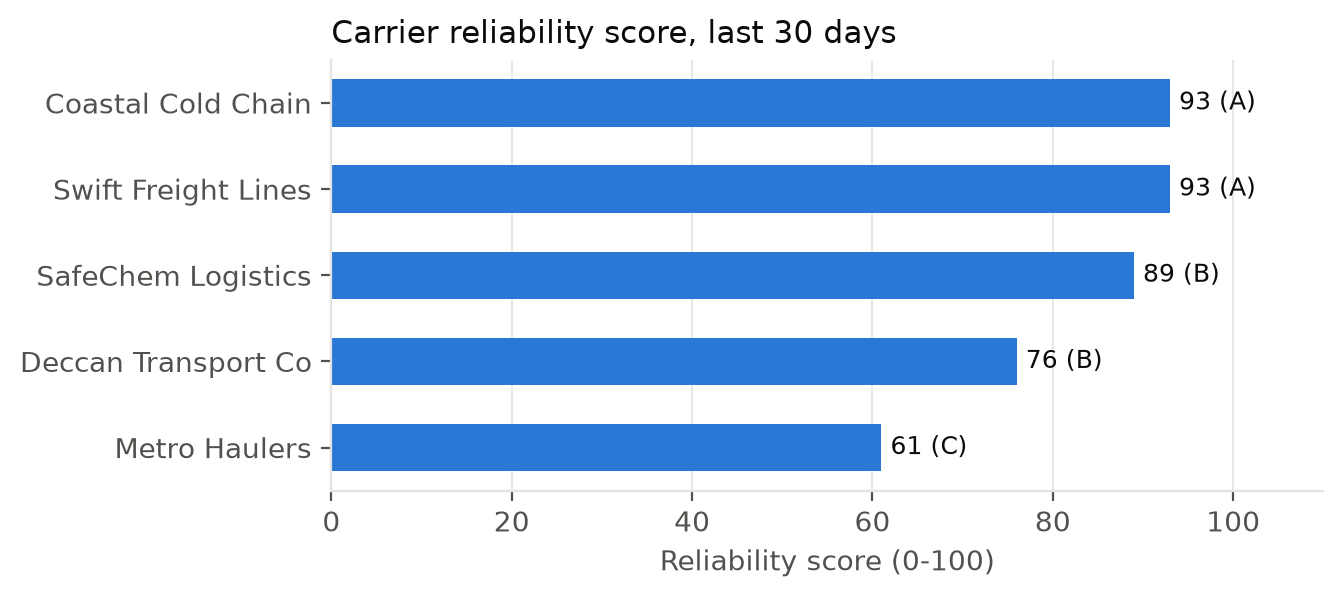
\includegraphics[width=\textwidth]{fig_carrier_reliability.png}
\end{columns}
\end{frame}

\begin{frame}{Results: Before vs.\ After (Simulation, 6 docks, 60 trucks/day, 60 days)}
\begin{columns}[c]
\column{0.5\textwidth}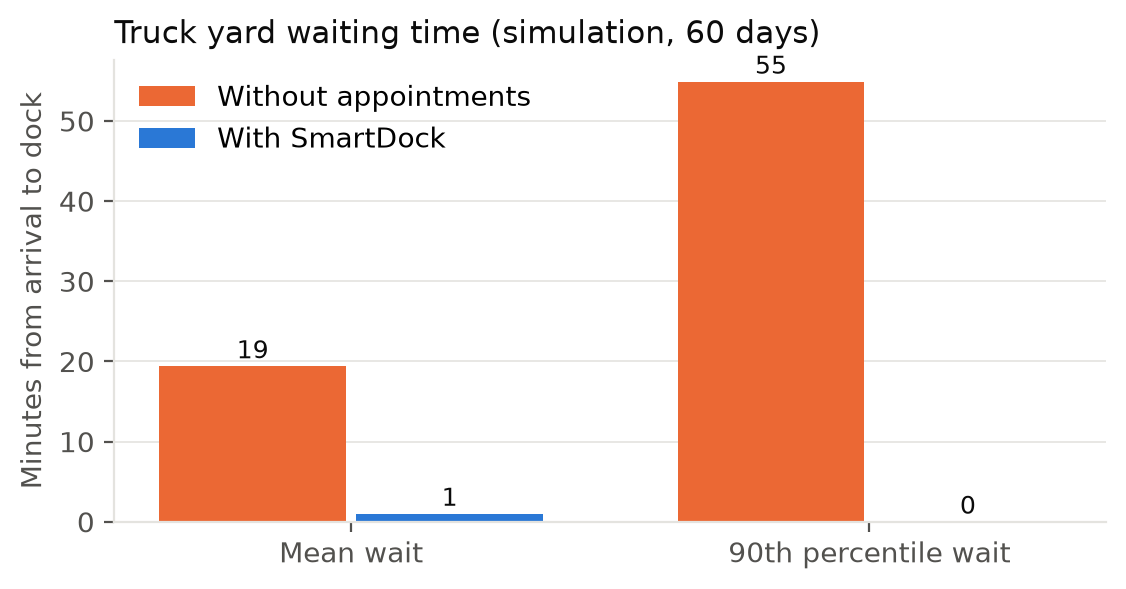
\includegraphics[width=\textwidth]{fig_sim_wait.png}
\column{0.5\textwidth}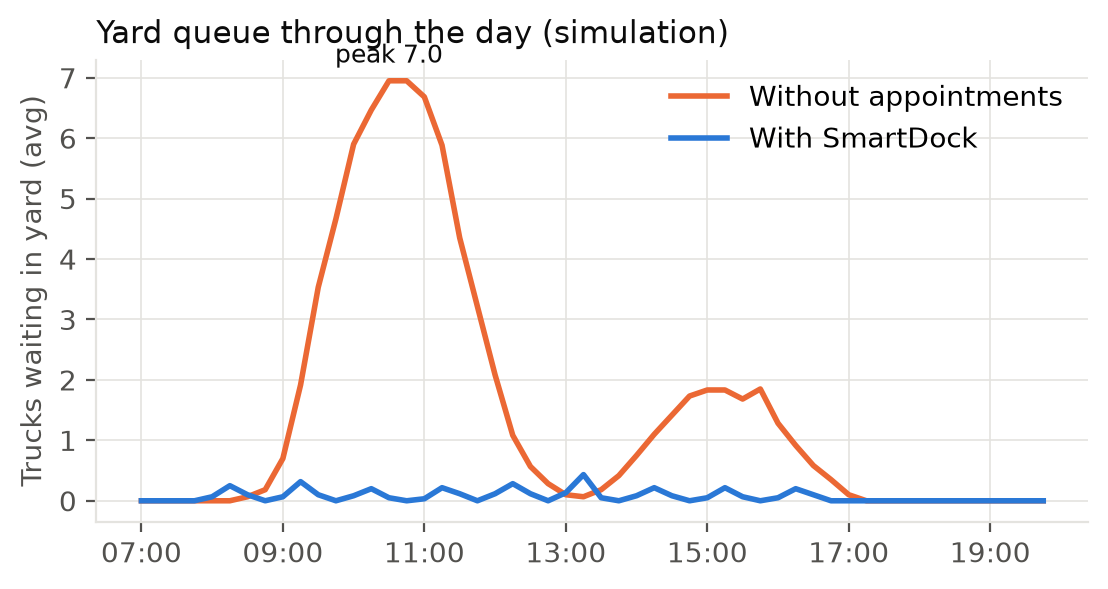
\includegraphics[width=\textwidth]{fig_sim_queue.png}
\end{columns}
\vspace{4pt}
\small
\centering
\begin{tabular}{lrr}
\toprule
& Without appointments & With SmartDock\\
\midrule
Mean yard wait & 19.4 min & \textbf{1.0 min}\\
Trucks waiting $>$ 30 min & 27.7\% & \textbf{0.3\%}\\
Peak yard queue & 7.0 trucks & \textbf{0.4 trucks}\\
\bottomrule
\end{tabular}
\end{frame}

% ================================================================ 25 benefits
\begin{frame}{Benefits and Real-World Applications}
\begin{columns}[T]
\column{0.55\textwidth}
\small
\begin{itemize}
  \item \textbf{Cost}: less detention and overtime; labour rostered to known load
  \item \textbf{Visibility}: one live schedule for both sides
  \item \textbf{Speed}: self-service booking; waiting $\approx$19 $\rightarrow$ $\approx$1 min (simulated)
  \item \textbf{Traceability}: PO/ASN, timestamps, full audit trail
  \item \textbf{Reliability}: conflict-free, hazmat-safe; carrier accountability
  \item \textbf{Sustainability}: less idling near the site
\end{itemize}
\column{0.42\textwidth}
\begin{block}{Applications}
\small Retail \& e-commerce DCs $\cdot$ cold-chain / pharma warehouses $\cdot$ chemical depots $\cdot$ 3PL multi-client sites $\cdot$ JIT manufacturing plants $\cdot$ container freight stations
\end{block}
\end{columns}
\end{frame}

% ================================================================ 26 conclusion
\begin{frame}{Conclusion}
\begin{itemize}
  \item Designed, built, tested and deployed a \alert{multi-tenant dock appointment and yard management system}
  \item All objectives met: configurable scheduling, dock matching, \alert{guaranteed capacity}, series, rescheduling, waitlist, yard events, reliability scores, KPIs, audit, notifications
  \item Verified by 58 automated checks and a concurrency experiment; live on the cloud
  \item A focused IT system at the warehouse--transport interface turns a phone-based process into a \alert{measured, collaborative} one
\end{itemize}
\end{frame}

% ================================================================ 27 future
\begin{frame}{Future Enhancements}
\begin{columns}[T]
\column{0.5\textwidth}
\begin{itemize}\small
  \item \textbf{AI/ML}: predict no-shows and delays; smart overbooking; volume forecasting
  \item \textbf{Optimisation}: automatic door assignment; load-based slot length
  \item \textbf{IoT}: ANPR / RFID gate check-in, dock sensors, reefer temperature
\end{itemize}
\column{0.5\textwidth}
\begin{itemize}\small
  \item \textbf{Integration}: ERP/WMS/TMS (PO, ASN), webhooks, carrier API
  \item \textbf{Mobile}: driver app / PWA with directions and proof of delivery
  \item \textbf{Scale}: WebSockets, analytics caching, Asian region, super-admin console, CI
\end{itemize}
\end{columns}
\end{frame}

% ================================================================ 28 references
\begin{frame}{References}
\scriptsize
\begin{enumerate}
  \item S.~Chopra, P.~Meindl, \emph{Supply Chain Management: Strategy, Planning, and Operation}, 6th ed., Pearson, 2016.
  \item M.~Christopher, \emph{Logistics \& Supply Chain Management}, 5th ed., Pearson, 2016.
  \item J.~Gu, M.~Goetschalckx, L.~F.~McGinnis, ``Research on warehouse operation: A comprehensive review,'' \emph{EJOR} 177(1), 2007.
  \item N.~Boysen, M.~Fliedner, ``Cross dock scheduling,'' \emph{Omega} 38(6), 2010.
  \item G.~Giuliano, T.~O'Brien, ``Reducing port-related truck emissions: The terminal gate appointment system \ldots,'' \emph{Transp.\ Res.\ D} 12(7), 2007.
  \item N.~Huynh, C.~M.~Walton, ``Robust scheduling of truck arrivals at marine container terminals,'' \emph{J.\ Transp.\ Eng.} 134(8), 2008.
  \item E.~Zehendner, D.~Feillet, ``Benefits of a truck appointment system \ldots,'' \emph{EJOR} 235(2), 2014.
  \item M.-H.~Phan, K.~H.~Kim, ``Negotiating truck arrival times \ldots,'' \emph{Transp.\ Res.\ E} 75, 2015.
  \item A.~M.~Law, \emph{Simulation Modeling and Analysis}, 5th ed., McGraw-Hill, 2015.
  \item M.~Kleppmann, \emph{Designing Data-Intensive Applications}, O'Reilly, 2017.
  \item MongoDB Manual --- Transactions; OWASP Top 10:2021; React, Express and Render documentation.
\end{enumerate}
\end{frame}

% ================================================================ 29 thanks
\begin{frame}[plain]
\begin{center}
\vspace{1.2cm}
{\Huge\bfseries\color{brand}Thank you}\\[0.4cm]
{\large Questions?}\\[0.8cm]
\small\url{\LiveURL}\quad$\cdot$\quad\url{\GitHubURL}\\[0.3cm]
\StudentName\ (\RegisterNumber)
\end{center}
\end{frame}

\end{document}
